\documentclass[border=3pt]{standalone}
% Preâmbulo compartilhado pelos diagramas TikZ da aula 12 (Mapeamento por Grade de Ocupação)
\usepackage[T1]{fontenc}
\usepackage[utf8]{inputenc}
\usepackage{lmodern}
\usepackage{amsmath}
\usepackage{xcolor}
\usepackage{tikz}
\usetikzlibrary{arrows.meta,angles,quotes,decorations.pathmorphing,calc,
                positioning,shapes.geometric,shapes.misc,backgrounds,fit,
                math}

% Paleta (mesma dos SVGs originais)
\definecolor{dblue}{HTML}{2A5B8C}
\definecolor{dorange}{HTML}{B3541E}
\definecolor{dgreen}{HTML}{4A7C59}
\definecolor{dred}{HTML}{9C4B4B}
\definecolor{dcream}{HTML}{F4F1EA}
\definecolor{dshade}{HTML}{DDD7C9}

% Função gaussiana (não normalizada por padrão de escala visual)
\pgfmathdeclarefunction{gauss}{3}{%
  \pgfmathparse{1/(#3*sqrt(2*pi))*exp(-((#1-#2)^2)/(2*#3^2))}%
}

% Estilos comuns (prefixo d... para não colidir com chaves internas do pgf)
\tikzset{
  >={Stealth[length=2mm]},
  dguide/.style={gray!55, dashed, line width=0.4pt},
  daxis/.style={gray!60, line width=0.7pt, ->},
  dbody/.style={fill=black!3, draw=black!80, line width=1pt},
  dacc/.style={draw=dblue, line width=1pt},
  dlbl/.style={black!55, font=\small},
  dsub/.style={black!45, font=\footnotesize},
  dstate/.style={circle, draw=black!80, fill=dcream, line width=1pt,
                 minimum size=17mm, font=\large, inner sep=1pt},
  dobs/.style={circle, draw=black!80, fill=dshade, line width=1pt,
               minimum size=14mm, font=\large, inner sep=1pt},
  dbox/.style={rounded corners=2pt, draw=black!80, fill=dcream, line width=1pt,
               align=center, inner sep=6pt},
  dop/.style={circle, draw=black!80, fill=white, line width=1pt,
              minimum size=6mm, inner sep=0pt, font=\small},
  dtrans/.style={->, dblue, line width=1pt},
  dmeas/.style={->, dorange, line width=1pt},
  dcurve/.style={line width=1pt, dblue},
  dcurveb/.style={line width=1.4pt, dorange},
}

\begin{document}
\hyphenpenalty=10000 \exhyphenpenalty=10000 \tolerance=9999 \emergencystretch=3em
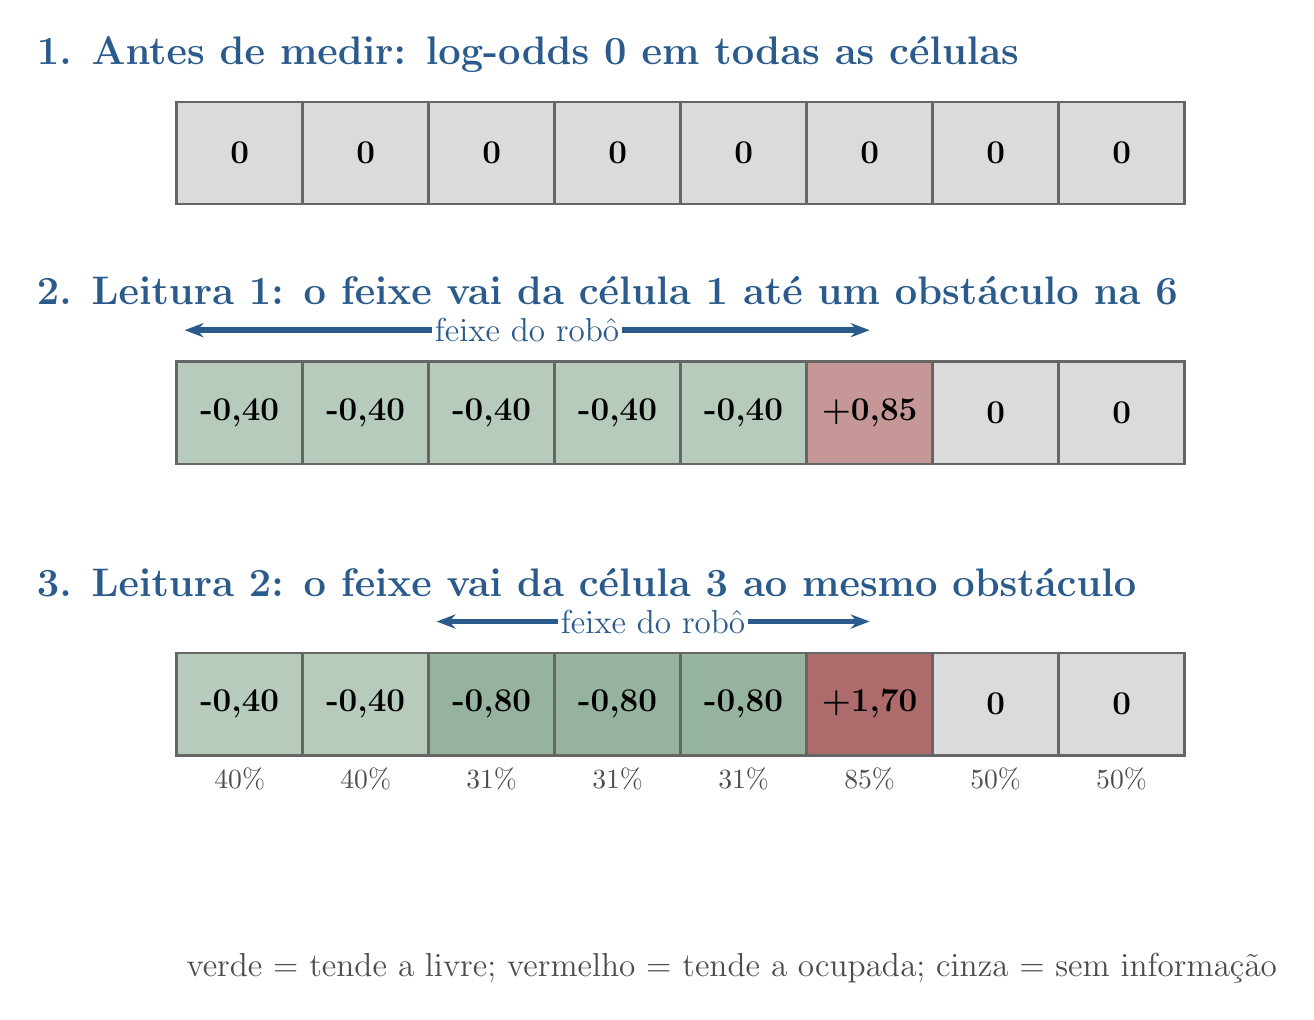
\begin{tikzpicture}[x=1cm,y=1cm]
  \node[font=\Large\bfseries, dblue, anchor=west] at (0,10.3) {1. Antes de medir: log-odds 0 em todas as células};
  \draw[black!60, line width=0.9pt, fill=black!14] (1.9,8.4) rectangle +(1.6,1.3);
  \node[font=\large\bfseries] at (2.7,9.05) {0};
  \draw[black!60, line width=0.9pt, fill=black!14] (3.5,8.4) rectangle +(1.6,1.3);
  \node[font=\large\bfseries] at (4.3,9.05) {0};
  \draw[black!60, line width=0.9pt, fill=black!14] (5.1,8.4) rectangle +(1.6,1.3);
  \node[font=\large\bfseries] at (5.9,9.05) {0};
  \draw[black!60, line width=0.9pt, fill=black!14] (6.700000000000001,8.4) rectangle +(1.6,1.3);
  \node[font=\large\bfseries] at (7.5,9.05) {0};
  \draw[black!60, line width=0.9pt, fill=black!14] (8.3,8.4) rectangle +(1.6,1.3);
  \node[font=\large\bfseries] at (9.1,9.05) {0};
  \draw[black!60, line width=0.9pt, fill=black!14] (9.9,8.4) rectangle +(1.6,1.3);
  \node[font=\large\bfseries] at (10.7,9.05) {0};
  \draw[black!60, line width=0.9pt, fill=black!14] (11.500000000000002,8.4) rectangle +(1.6,1.3);
  \node[font=\large\bfseries] at (12.3,9.05) {0};
  \draw[black!60, line width=0.9pt, fill=black!14] (13.100000000000001,8.4) rectangle +(1.6,1.3);
  \node[font=\large\bfseries] at (13.9,9.05) {0};
  \node[font=\Large\bfseries, dblue, anchor=west] at (0,7.3) {2. Leitura 1: o feixe vai da célula 1 até um obstáculo na 6};
  \draw[black!60, line width=0.9pt, fill=dgreen!40] (1.9,5.1) rectangle +(1.6,1.3);
  \node[font=\large\bfseries] at (2.7,5.75) {-0,40};
  \draw[black!60, line width=0.9pt, fill=dgreen!40] (3.5,5.1) rectangle +(1.6,1.3);
  \node[font=\large\bfseries] at (4.3,5.75) {-0,40};
  \draw[black!60, line width=0.9pt, fill=dgreen!40] (5.1,5.1) rectangle +(1.6,1.3);
  \node[font=\large\bfseries] at (5.9,5.75) {-0,40};
  \draw[black!60, line width=0.9pt, fill=dgreen!40] (6.700000000000001,5.1) rectangle +(1.6,1.3);
  \node[font=\large\bfseries] at (7.5,5.75) {-0,40};
  \draw[black!60, line width=0.9pt, fill=dgreen!40] (8.3,5.1) rectangle +(1.6,1.3);
  \node[font=\large\bfseries] at (9.1,5.75) {-0,40};
  \draw[black!60, line width=0.9pt, fill=dred!58] (9.9,5.1) rectangle +(1.6,1.3);
  \node[font=\large\bfseries] at (10.7,5.75) {+0,85};
  \draw[black!60, line width=0.9pt, fill=black!14] (11.500000000000002,5.1) rectangle +(1.6,1.3);
  \node[font=\large\bfseries] at (12.3,5.75) {0};
  \draw[black!60, line width=0.9pt, fill=black!14] (13.100000000000001,5.1) rectangle +(1.6,1.3);
  \node[font=\large\bfseries] at (13.9,5.75) {0};
  \draw[dblue, line width=2pt, <->, >={Stealth[length=2.4mm]}] (2.0,6.8) -- (10.7,6.8);
  \node[font=\large, dblue, fill=white, inner sep=1pt] at (6.35,6.8) {feixe do robô};
  \node[font=\Large\bfseries, dblue, anchor=west] at (0,3.6) {3. Leitura 2: o feixe vai da célula 3 ao mesmo obstáculo};
  \draw[black!60, line width=0.9pt, fill=dgreen!40] (1.9,1.4) rectangle +(1.6,1.3);
  \node[font=\large\bfseries] at (2.7,2.05) {-0,40};
  \node[font=\normalsize, black!70] at (2.7,1.1) {40\%};
  \draw[black!60, line width=0.9pt, fill=dgreen!40] (3.5,1.4) rectangle +(1.6,1.3);
  \node[font=\large\bfseries] at (4.3,2.05) {-0,40};
  \node[font=\normalsize, black!70] at (4.3,1.1) {40\%};
  \draw[black!60, line width=0.9pt, fill=dgreen!58] (5.1,1.4) rectangle +(1.6,1.3);
  \node[font=\large\bfseries] at (5.9,2.05) {-0,80};
  \node[font=\normalsize, black!70] at (5.9,1.1) {31\%};
  \draw[black!60, line width=0.9pt, fill=dgreen!58] (6.700000000000001,1.4) rectangle +(1.6,1.3);
  \node[font=\large\bfseries] at (7.5,2.05) {-0,80};
  \node[font=\normalsize, black!70] at (7.5,1.1) {31\%};
  \draw[black!60, line width=0.9pt, fill=dgreen!58] (8.3,1.4) rectangle +(1.6,1.3);
  \node[font=\large\bfseries] at (9.1,2.05) {-0,80};
  \node[font=\normalsize, black!70] at (9.1,1.1) {31\%};
  \draw[black!60, line width=0.9pt, fill=dred!82] (9.9,1.4) rectangle +(1.6,1.3);
  \node[font=\large\bfseries] at (10.7,2.05) {+1,70};
  \node[font=\normalsize, black!70] at (10.7,1.1) {85\%};
  \draw[black!60, line width=0.9pt, fill=black!14] (11.500000000000002,1.4) rectangle +(1.6,1.3);
  \node[font=\large\bfseries] at (12.3,2.05) {0};
  \node[font=\normalsize, black!70] at (12.3,1.1) {50\%};
  \draw[black!60, line width=0.9pt, fill=black!14] (13.100000000000001,1.4) rectangle +(1.6,1.3);
  \node[font=\large\bfseries] at (13.9,2.05) {0};
  \node[font=\normalsize, black!70] at (13.9,1.1) {50\%};
  \draw[dblue, line width=2pt, <->, >={Stealth[length=2.4mm]}] (5.2,3.1) -- (10.7,3.1);
  \node[font=\large, dblue, fill=white, inner sep=1pt] at (7.95,3.1) {feixe do robô};
  \node[font=\large, black!70, anchor=west] at (1.9,-1.3) {verde = tende a livre; vermelho = tende a ocupada; cinza = sem informação};
\end{tikzpicture}
\end{document}
